% Options for packages loaded elsewhere
\PassOptionsToPackage{unicode}{hyperref}
\PassOptionsToPackage{hyphens}{url}
%
\documentclass[
]{article}
\usepackage{amsmath,amssymb}
\usepackage{iftex}
\ifPDFTeX
  \usepackage[T1]{fontenc}
  \usepackage[utf8]{inputenc}
  \usepackage{textcomp} % provide euro and other symbols
\else % if luatex or xetex
  \usepackage{unicode-math} % this also loads fontspec
  \defaultfontfeatures{Scale=MatchLowercase}
  \defaultfontfeatures[\rmfamily]{Ligatures=TeX,Scale=1}
\fi
\usepackage{lmodern}
\ifPDFTeX\else
  % xetex/luatex font selection
\fi
% Use upquote if available, for straight quotes in verbatim environments
\IfFileExists{upquote.sty}{\usepackage{upquote}}{}
\IfFileExists{microtype.sty}{% use microtype if available
  \usepackage[]{microtype}
  \UseMicrotypeSet[protrusion]{basicmath} % disable protrusion for tt fonts
}{}
\makeatletter
\@ifundefined{KOMAClassName}{% if non-KOMA class
  \IfFileExists{parskip.sty}{%
    \usepackage{parskip}
  }{% else
    \setlength{\parindent}{0pt}
    \setlength{\parskip}{6pt plus 2pt minus 1pt}}
}{% if KOMA class
  \KOMAoptions{parskip=half}}
\makeatother
\usepackage{xcolor}
\usepackage[margin=1in]{geometry}
\usepackage{color}
\usepackage{fancyvrb}
\newcommand{\VerbBar}{|}
\newcommand{\VERB}{\Verb[commandchars=\\\{\}]}
\DefineVerbatimEnvironment{Highlighting}{Verbatim}{commandchars=\\\{\}}
% Add ',fontsize=\small' for more characters per line
\usepackage{framed}
\definecolor{shadecolor}{RGB}{248,248,248}
\newenvironment{Shaded}{\begin{snugshade}}{\end{snugshade}}
\newcommand{\AlertTok}[1]{\textcolor[rgb]{0.94,0.16,0.16}{#1}}
\newcommand{\AnnotationTok}[1]{\textcolor[rgb]{0.56,0.35,0.01}{\textbf{\textit{#1}}}}
\newcommand{\AttributeTok}[1]{\textcolor[rgb]{0.13,0.29,0.53}{#1}}
\newcommand{\BaseNTok}[1]{\textcolor[rgb]{0.00,0.00,0.81}{#1}}
\newcommand{\BuiltInTok}[1]{#1}
\newcommand{\CharTok}[1]{\textcolor[rgb]{0.31,0.60,0.02}{#1}}
\newcommand{\CommentTok}[1]{\textcolor[rgb]{0.56,0.35,0.01}{\textit{#1}}}
\newcommand{\CommentVarTok}[1]{\textcolor[rgb]{0.56,0.35,0.01}{\textbf{\textit{#1}}}}
\newcommand{\ConstantTok}[1]{\textcolor[rgb]{0.56,0.35,0.01}{#1}}
\newcommand{\ControlFlowTok}[1]{\textcolor[rgb]{0.13,0.29,0.53}{\textbf{#1}}}
\newcommand{\DataTypeTok}[1]{\textcolor[rgb]{0.13,0.29,0.53}{#1}}
\newcommand{\DecValTok}[1]{\textcolor[rgb]{0.00,0.00,0.81}{#1}}
\newcommand{\DocumentationTok}[1]{\textcolor[rgb]{0.56,0.35,0.01}{\textbf{\textit{#1}}}}
\newcommand{\ErrorTok}[1]{\textcolor[rgb]{0.64,0.00,0.00}{\textbf{#1}}}
\newcommand{\ExtensionTok}[1]{#1}
\newcommand{\FloatTok}[1]{\textcolor[rgb]{0.00,0.00,0.81}{#1}}
\newcommand{\FunctionTok}[1]{\textcolor[rgb]{0.13,0.29,0.53}{\textbf{#1}}}
\newcommand{\ImportTok}[1]{#1}
\newcommand{\InformationTok}[1]{\textcolor[rgb]{0.56,0.35,0.01}{\textbf{\textit{#1}}}}
\newcommand{\KeywordTok}[1]{\textcolor[rgb]{0.13,0.29,0.53}{\textbf{#1}}}
\newcommand{\NormalTok}[1]{#1}
\newcommand{\OperatorTok}[1]{\textcolor[rgb]{0.81,0.36,0.00}{\textbf{#1}}}
\newcommand{\OtherTok}[1]{\textcolor[rgb]{0.56,0.35,0.01}{#1}}
\newcommand{\PreprocessorTok}[1]{\textcolor[rgb]{0.56,0.35,0.01}{\textit{#1}}}
\newcommand{\RegionMarkerTok}[1]{#1}
\newcommand{\SpecialCharTok}[1]{\textcolor[rgb]{0.81,0.36,0.00}{\textbf{#1}}}
\newcommand{\SpecialStringTok}[1]{\textcolor[rgb]{0.31,0.60,0.02}{#1}}
\newcommand{\StringTok}[1]{\textcolor[rgb]{0.31,0.60,0.02}{#1}}
\newcommand{\VariableTok}[1]{\textcolor[rgb]{0.00,0.00,0.00}{#1}}
\newcommand{\VerbatimStringTok}[1]{\textcolor[rgb]{0.31,0.60,0.02}{#1}}
\newcommand{\WarningTok}[1]{\textcolor[rgb]{0.56,0.35,0.01}{\textbf{\textit{#1}}}}
\usepackage{graphicx}
\makeatletter
\def\maxwidth{\ifdim\Gin@nat@width>\linewidth\linewidth\else\Gin@nat@width\fi}
\def\maxheight{\ifdim\Gin@nat@height>\textheight\textheight\else\Gin@nat@height\fi}
\makeatother
% Scale images if necessary, so that they will not overflow the page
% margins by default, and it is still possible to overwrite the defaults
% using explicit options in \includegraphics[width, height, ...]{}
\setkeys{Gin}{width=\maxwidth,height=\maxheight,keepaspectratio}
% Set default figure placement to htbp
\makeatletter
\def\fps@figure{htbp}
\makeatother
\setlength{\emergencystretch}{3em} % prevent overfull lines
\providecommand{\tightlist}{%
  \setlength{\itemsep}{0pt}\setlength{\parskip}{0pt}}
\setcounter{secnumdepth}{-\maxdimen} % remove section numbering
\ifLuaTeX
  \usepackage{selnolig}  % disable illegal ligatures
\fi
\usepackage{bookmark}
\IfFileExists{xurl.sty}{\usepackage{xurl}}{} % add URL line breaks if available
\urlstyle{same}
\hypersetup{
  pdftitle={Analysis of Categorical Data (cont.)},
  pdfauthor={NRES 710},
  hidelinks,
  pdfcreator={LaTeX via pandoc}}

\title{Analysis of Categorical Data (cont.)}
\author{NRES 710}
\date{Last compiled: 2024-08-19}

\begin{document}
\maketitle

\subsection{Summary}\label{summary}

Last class we discussed how to analyze data when we have a categorical
X-variable data.

Traditionally, this is called a \emph{t-test} -- but I am going to avoid
calling it that going forward. Instead, we are always going to be using
the \textbf{linear model} in this class, which is more
\emph{parsimonious} (simple) and will create continuity with the
approach we are going to take toward understanding statistics in this
class

Today we will discuss how to \textbf{present results} from analysis of
categorical data. We have a `canned' sentence for presenting results
when we have two continuous variables, but we need a slightly different
approach for when we have categorical X-data.

The good news is that our X-variable data can only be continuous or
categorical. So once we learn this second approach, we will only have to
know these \textbf{two approaches}. We can use them repeatedly during
our various analytical activities, perhaps with slight modifications.

\subsection{Presenting Results}\label{presenting-results}

With continuous X data, we start out by saying: ``For each 1 unit
increase in X, we observed a unit change in Y.'' There is no such thing
as a unit change in X when we have a categorical X variable, so we will
drop that. Instead, we will say something like:

**``We found that {[}group 1{]} was {[}\(\beta_1\){]} {[}Y-units{]}
({[}+/-CI{]}; 95\% CI) {[}descriptor word to indicate direction{]} than
{[}group 2{]} (p = {[}p-value{]}).''

\begin{itemize}
\tightlist
\item
  *if p \textgreater{} 0.05, then add: ``; however, our results were not
  statistically significant.''
\end{itemize}

\subsubsection{Example}\label{example}

Let's take a peak in R at the elephant
\href{lecture_8_seal_data.csv}{seal body size data} from last class. We
will analyze it using `lm()' with a categorical X-variable:

\begin{Shaded}
\begin{Highlighting}[]
\CommentTok{\# Load the data}
\NormalTok{datum }\OtherTok{\textless{}{-}} \FunctionTok{read.csv}\NormalTok{(}\StringTok{"lecture\_8\_seal\_data.csv"}\NormalTok{)}

\CommentTok{\# Examine it}
\FunctionTok{head}\NormalTok{(datum)}
\FunctionTok{tail}\NormalTok{(datum)}

\CommentTok{\# Examine structure of data}
\FunctionTok{str}\NormalTok{(datum)}
\end{Highlighting}
\end{Shaded}

\begin{verbatim}
## 'data.frame':    40 obs. of  4 variables:
##  $ X   : int  1 2 3 4 5 6 7 8 9 10 ...
##  $ Sex : chr  "Female" "Female" "Female" "Female" ...
##  $ Size: num  189 195 231 201 203 ...
##  $ Male: int  0 0 0 0 0 0 0 0 0 0 ...
\end{verbatim}

\begin{Shaded}
\begin{Highlighting}[]
\CommentTok{\# Force \textquotesingle{}Sex\textquotesingle{} to be a factor}
\NormalTok{datum}\SpecialCharTok{$}\NormalTok{Sex }\OtherTok{\textless{}{-}} \FunctionTok{factor}\NormalTok{(datum}\SpecialCharTok{$}\NormalTok{Sex)}

\CommentTok{\# Scatterplot}
\FunctionTok{plot}\NormalTok{(Size }\SpecialCharTok{\textasciitilde{}}\NormalTok{ Sex, }\AttributeTok{data =}\NormalTok{ datum)}
\end{Highlighting}
\end{Shaded}

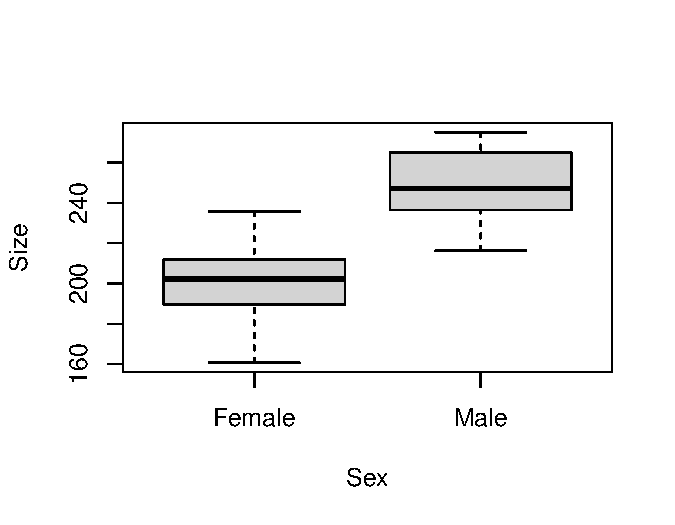
\includegraphics{lecture_9_files/figure-latex/seals-1.pdf}

\begin{Shaded}
\begin{Highlighting}[]
\CommentTok{\# Fit a linear model}
\NormalTok{results }\OtherTok{\textless{}{-}} \FunctionTok{lm}\NormalTok{(Size }\SpecialCharTok{\textasciitilde{}}\NormalTok{ Sex, }\AttributeTok{data =}\NormalTok{ datum)}
\FunctionTok{summary}\NormalTok{(results)}
\end{Highlighting}
\end{Shaded}

\begin{verbatim}
## 
## Call:
## lm(formula = Size ~ Sex, data = datum)
## 
## Residuals:
##    Min     1Q Median     3Q    Max 
## -42.16 -12.60  -0.43  12.78  32.91 
## 
## Coefficients:
##             Estimate Std. Error t value Pr(>|t|)    
## (Intercept)   202.83       4.04   50.16  < 2e-16 ***
## SexMale        46.14       5.72    8.07  9.2e-10 ***
## ---
## Signif. codes:  0 '***' 0.001 '**' 0.01 '*' 0.05 '.' 0.1 ' ' 1
## 
## Residual standard error: 18.1 on 38 degrees of freedom
## Multiple R-squared:  0.631,  Adjusted R-squared:  0.622 
## F-statistic: 65.1 on 1 and 38 DF,  p-value: 9.24e-10
\end{verbatim}

Let's talk about this a bit to make sure we are all on the same page.

The analysis output from linear regression with \textbf{categorical
X-data} is the same output that we got when we ran linear regression
using \textbf{two continuous variables}.

\begin{itemize}
\tightlist
\item
  \(\beta_0\) -- the Y-intercept; previously this was the value when Y =
  0; now it is slightly different, it is still the Y-value when X = 0,
  but we can more technically define this as the average Y-value for the
  `reference group'.

  \begin{itemize}
  \tightlist
  \item
    We get to choose what the reference group is. By default, R chose
    `female' as the reference group, and we can see that because
    `SexMale' was the \(\beta_1\) effect.
  \end{itemize}
\item
  \(\beta_1\) -- the difference in size between males and females. The
  \textbf{p-value} is testing the null hypothesis that there is no
  difference in size between males and females.
\item
  Residual standard error -- noise around the average
\item
  Everything else is still the same
\end{itemize}

We can now use this output to populate the our `presenting resultings'
sentence. We will need the +/- 95\% CI:

\begin{Shaded}
\begin{Highlighting}[]
\CommentTok{\# Confidence intervals}
\FunctionTok{confint}\NormalTok{(results)}
\end{Highlighting}
\end{Shaded}

\begin{verbatim}
##              2.5 % 97.5 %
## (Intercept) 194.65 211.02
## SexMale      34.57  57.72
\end{verbatim}

\begin{Shaded}
\begin{Highlighting}[]
\CommentTok{\# Calculate confidence intervals}
\FloatTok{57.7} \SpecialCharTok{{-}} \FloatTok{46.1}
\end{Highlighting}
\end{Shaded}

\begin{verbatim}
## [1] 11.6
\end{verbatim}

\begin{Shaded}
\begin{Highlighting}[]
\CommentTok{\# simple way: upper limit minus mean}
\FunctionTok{confint}\NormalTok{(results)[}\StringTok{"SexMale"}\NormalTok{, }\DecValTok{2}\NormalTok{] }\SpecialCharTok{{-}}\NormalTok{ results}\SpecialCharTok{$}\NormalTok{coefficients[}\StringTok{"SexMale"}\NormalTok{]}
\end{Highlighting}
\end{Shaded}

\begin{verbatim}
## SexMale 
##   11.58
\end{verbatim}

\begin{Shaded}
\begin{Highlighting}[]
\CommentTok{\# extracting estimates from objects to do math}
\end{Highlighting}
\end{Shaded}

\textbf{``We found that males were 46.1 kg (+/-11.6; +/-95\% CI) heavier
than females (p = 9.24e-10).''}

You could also be more descriptive and perhaps say: ``had 46.1 kg
(\ldots) greater mass than females''. It's nice to be descriptive -- but
also good to keep things concise.

What if you wanted to put females first? That's fine -- just swap things
around, word smith it a bit, and put females first: ``We found that
females had 46.1 kg (\ldots) less mass than males''.

If you give R categorical data, R will automatically create the
`reference' group using the alphabetical order of the groups. For
example, if you gave R data with two experimental treatments in the
X-variable, ``control'' and ``burned'', it will automatically make
``burned'' the reference group -- but you might want to change that to
visualize the `effect' of burn treatment compared to control, untreated
areas.

\textbf{Takehome message:} Running a t-test is the same as running a
regression, but with a categorical X-variable -- but it doesn't matter
with coding in R. The only difference is you have to understand that you
have a categorical X-variable, and write a slightly different sentence.

\subsubsection{Changing the reference
group}\label{changing-the-reference-group}

We can change what the reference group is in R using the `factor()'
function. For example, using our seal data:

\begin{Shaded}
\begin{Highlighting}[]
\CommentTok{\# Examine the categorical data}
\FunctionTok{str}\NormalTok{(datum}\SpecialCharTok{$}\NormalTok{Sex)}
\end{Highlighting}
\end{Shaded}

\begin{verbatim}
##  Factor w/ 2 levels "Female","Male": 1 1 1 1 1 1 1 1 1 1 ...
\end{verbatim}

\begin{Shaded}
\begin{Highlighting}[]
\CommentTok{\# The \textquotesingle{}levels\textquotesingle{} are the groups in the variable, and they are ordered alphabetically by default.}

\CommentTok{\# Re{-}order the levels}
\NormalTok{datum}\SpecialCharTok{$}\NormalTok{Sex }\OtherTok{\textless{}{-}} \FunctionTok{factor}\NormalTok{(datum}\SpecialCharTok{$}\NormalTok{Sex, }\AttributeTok{levels =} \FunctionTok{c}\NormalTok{(}\StringTok{"Male"}\NormalTok{, }\StringTok{"Female"}\NormalTok{)) }\CommentTok{\# switch the order}

\CommentTok{\# Re{-}run model}
\NormalTok{results2 }\OtherTok{\textless{}{-}} \FunctionTok{lm}\NormalTok{(Size }\SpecialCharTok{\textasciitilde{}}\NormalTok{ Sex, }\AttributeTok{data =}\NormalTok{ datum)}
\FunctionTok{summary}\NormalTok{(results2)}
\end{Highlighting}
\end{Shaded}

\begin{verbatim}
## 
## Call:
## lm(formula = Size ~ Sex, data = datum)
## 
## Residuals:
##    Min     1Q Median     3Q    Max 
## -42.16 -12.60  -0.43  12.78  32.91 
## 
## Coefficients:
##             Estimate Std. Error t value Pr(>|t|)    
## (Intercept)   248.97       4.04   61.58  < 2e-16 ***
## SexFemale     -46.14       5.72   -8.07  9.2e-10 ***
## ---
## Signif. codes:  0 '***' 0.001 '**' 0.01 '*' 0.05 '.' 0.1 ' ' 1
## 
## Residual standard error: 18.1 on 38 degrees of freedom
## Multiple R-squared:  0.631,  Adjusted R-squared:  0.622 
## F-statistic: 65.1 on 1 and 38 DF,  p-value: 9.24e-10
\end{verbatim}

Now `SexFemale' is the \(\beta_1\) effect.

\subsection{Multiple groups}\label{multiple-groups}

Let's extend this model a little bit. Previously we had considered a
situation where we had a `binomial' X-variable (\emph{bi-} and
\emph{nomial} = \emph{two} \emph{names} = a categorical variable with
two categories). Let's now consider a situation where we have a
multinomial (\emph{multi-} = more than two) X-variable with more than
two categories within it.

\textbf{Continuous Y; Multinomial X}

\begin{itemize}
\tightlist
\item
  \textbf{X-variable: Group 1 - Juveniles, Group 2 - Subadults, Group 3
  - Adults}
\item
  \textbf{Y-variable: body size (mass)}
\end{itemize}

The first thing I want to show you is how this works in the general
linear modeling framework. Up to this point, we have used our trusty
equation for the linear model as:

\textbf{\(Y = \beta_0 + \beta_1 X_1 + \epsilon \sim N(0, \sigma)\)}

We previously introduced the concept of `dummy coding', which will be
particularly useful for us to explain how to extend our simple linear
model to accommodate multiple groups.

We will take our categorical X-variable and `dummy code' it by creating
a \textbf{column for each category} that describes whether each
observation in our data is \textbf{within that category (1) or not (0)}.
For example:

When we create our general linear model to accommodate these multiple
groups, we now need to have an X for every one of these dummy-coded
columns. But, we are going to leave one out.

\textbf{\(Y = \beta_0 + \beta_1 Subadult + \beta_2 Adult + \epsilon \sim N(0, \sigma)\)}

You might be scratching your head why `Juvenile' wasn't included. We
don't need to include it because it will be automatically be captured by
the \(\beta_0\) intercept!

\begin{itemize}
\tightlist
\item
  Subadults will be captured by the \(\beta_1 Subadult\) term.
\item
  Adults will be captured by the \(\beta_2 Adult\) term.
\item
  So then Juveniles will be all the individuals that weren't in Subadult
  or Adults categories and thus will captured by the intercept as the
  `reference' group.
\end{itemize}

The reference group is the group by which all others are compared.

Another way to look at this is to examine our dummy-coded columns. If we
look at the `Subadult' and `Adult' columns, we actually don't need the
`Juvenile' column to know which observations are of juveniles:

The individuals that were 0 for both Subadults and Adults must be
Juveniles, by the process of elimination.

\textbf{Let's see how this works mathematically:}

\textbf{\(Y = \beta_0 + \beta_1 Subadult + \beta_2 Adult + \epsilon\)}

\textbf{\(Y(juv) = \beta_0 + \cancel{\beta_1 * 0} + \cancel{\beta_2 * 0} + \epsilon\)}

\textbf{\(Y(juv) = \beta_0 + \epsilon\)}

The meaning of \(\beta_0\) has not changed -- the average Y (size) of
our reference group.

\textbf{\(Y(sub) = \beta_0 + \beta_1 * 1 + \cancel{\beta_2 * 0} + \epsilon\)}

\textbf{\(Y(sub) = \beta_0 + \beta_1 + \epsilon\)}

The meaning of \(\beta_1\) has not changed either -- the difference
between juveniles and subadults.

\textbf{\(Y(adult) = \beta_0 + \cancel{\beta_1 * 0} + \beta_2 * 1 + \epsilon\)}

\textbf{\(Y(adult) = \beta_0 + \beta_2 + \epsilon\)}

Our new variable, \(\beta_2\), has a similar meaning to \(\beta_1\) --
the difference between adults and juveniles.

I like to visualize these things \textbf{graphically}. So I am going to
draw something that might help us visualize this on the board:

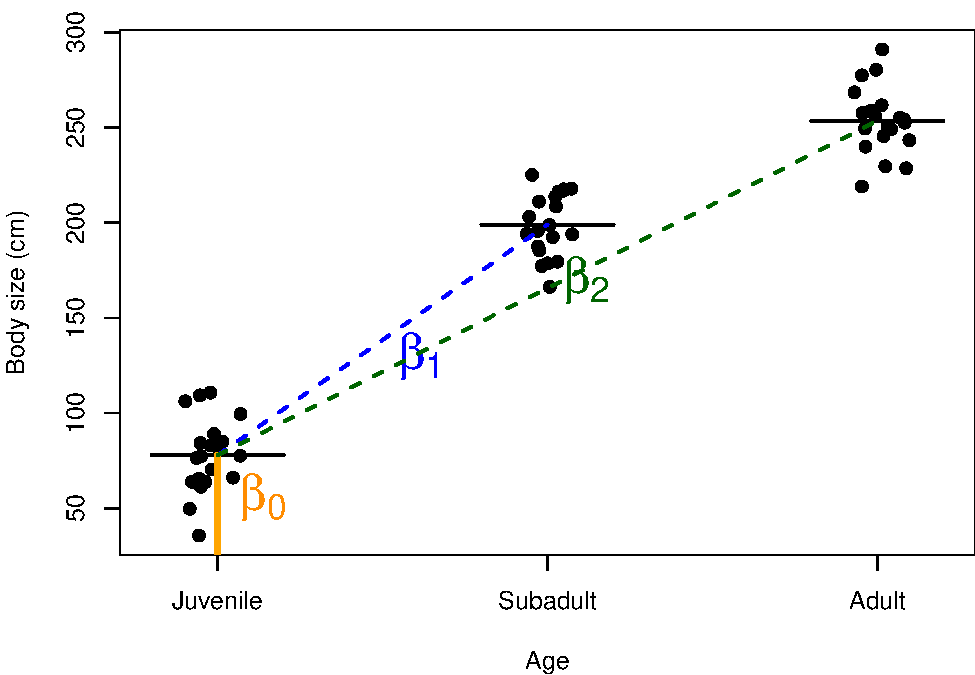
\includegraphics{lecture_9_files/figure-latex/stripplot-1.pdf}

Note: our \textbf{error} is normally distributed with a mean = 0,
centered on the average, with a standard deviation of \(\sigma\).

Or:

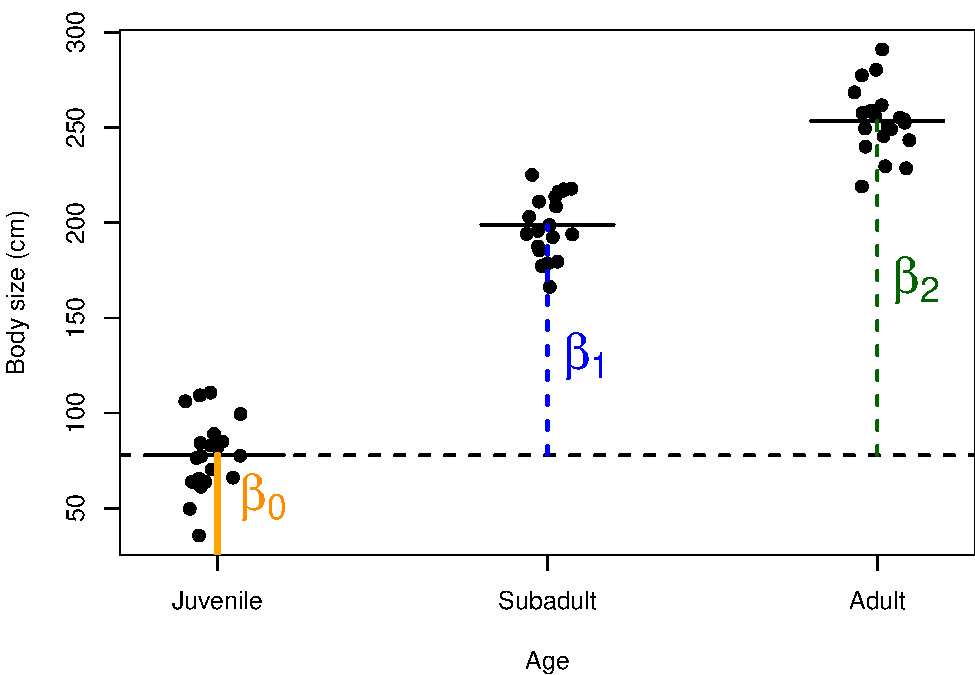
\includegraphics{lecture_9_files/figure-latex/stripplot-2-1.pdf}

\textbf{Q:} Does anyone have any questions?

You might be wondering\ldots{} how would we estimate the difference
between subadults and adults?

\begin{itemize}
\tightlist
\item
  \(\beta_1\) tells us about the difference between juveniles and
  subadults, and whether it's statistically significant.
\item
  \(\beta_2\) tells us about the difference between juveniles and
  adults, and whether it's statistically significant.
\item
  But neither tells us about the difference between juveniles and
  adults.
\end{itemize}

\textbf{Q:} Anybody know how we might learn about the difference between
juveniles and adults? \textbf{Changing the reference.}

\subsubsection{Comparison of multiple groups in
R}\label{comparison-of-multiple-groups-in-r}

Let's see what this would look like in R. Download some simulated data
\href{lecture_9_ages.csv}{here}.

\begin{Shaded}
\begin{Highlighting}[]
\DocumentationTok{\#\#\# Code to test for differences among three groups}

\CommentTok{\# Read in the data}
\NormalTok{datum }\OtherTok{\textless{}{-}} \FunctionTok{read.csv}\NormalTok{(}\StringTok{"lecture\_9\_ages.csv"}\NormalTok{)}

\CommentTok{\# Examine the data}
\FunctionTok{head}\NormalTok{(datum)}

\CommentTok{\# Plot}
\FunctionTok{stripchart}\NormalTok{(Size }\SpecialCharTok{\textasciitilde{}}\NormalTok{ Age, }\AttributeTok{data =}\NormalTok{ datum, }\AttributeTok{vertical =} \ConstantTok{TRUE}\NormalTok{, }\AttributeTok{method =} \StringTok{"jitter"}\NormalTok{,}
           \AttributeTok{pch =} \DecValTok{19}\NormalTok{, }\AttributeTok{xlab =} \StringTok{"Age"}\NormalTok{, }\AttributeTok{ylab =} \StringTok{"Body size (cm)"}\NormalTok{)}
\end{Highlighting}
\end{Shaded}

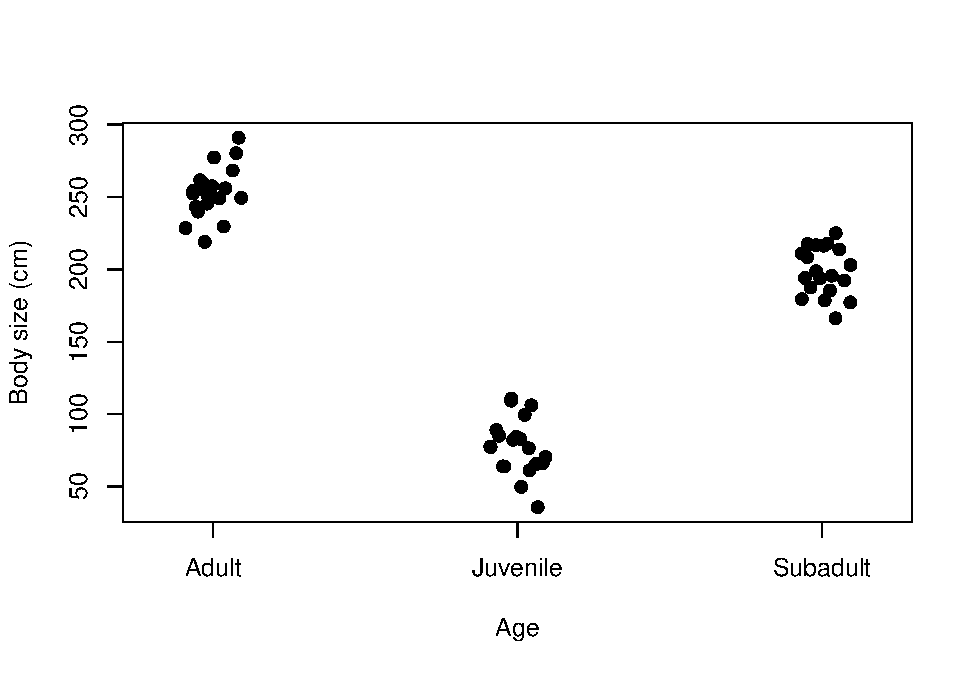
\includegraphics{lecture_9_files/figure-latex/three-groups-analysis-1.pdf}

\begin{Shaded}
\begin{Highlighting}[]
\CommentTok{\# Re{-}order categorical X{-}data}
\NormalTok{datum}\SpecialCharTok{$}\NormalTok{Age }\OtherTok{\textless{}{-}} \FunctionTok{factor}\NormalTok{(datum}\SpecialCharTok{$}\NormalTok{Age, }\AttributeTok{levels =} \FunctionTok{c}\NormalTok{(}\StringTok{"Juvenile"}\NormalTok{, }\StringTok{"Subadult"}\NormalTok{, }\StringTok{"Adult"}\NormalTok{))}

\CommentTok{\# Plot}
\FunctionTok{stripchart}\NormalTok{(Size }\SpecialCharTok{\textasciitilde{}}\NormalTok{ Age, }\AttributeTok{data =}\NormalTok{ datum, }\AttributeTok{vertical =} \ConstantTok{TRUE}\NormalTok{, }\AttributeTok{method =} \StringTok{"jitter"}\NormalTok{,}
           \AttributeTok{pch =} \DecValTok{19}\NormalTok{, }\AttributeTok{xlab =} \StringTok{"Age"}\NormalTok{, }\AttributeTok{ylab =} \StringTok{"Body size (cm)"}\NormalTok{)}
\end{Highlighting}
\end{Shaded}

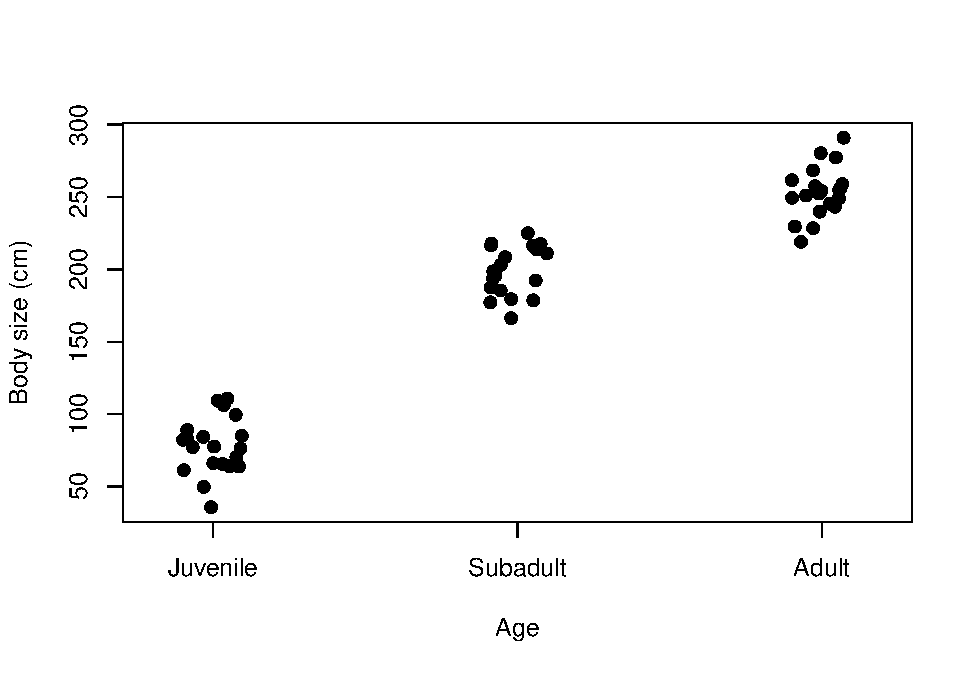
\includegraphics{lecture_9_files/figure-latex/three-groups-analysis-2.pdf}

\begin{Shaded}
\begin{Highlighting}[]
\CommentTok{\# Add in dummy{-}coding}
\NormalTok{dummy }\OtherTok{\textless{}{-}} \FunctionTok{model.matrix}\NormalTok{(}\SpecialCharTok{\textasciitilde{}}\NormalTok{ Age }\SpecialCharTok{{-}}\DecValTok{1}\NormalTok{, }\AttributeTok{data =}\NormalTok{ datum)}
\FunctionTok{colnames}\NormalTok{(dummy) }\OtherTok{\textless{}{-}} \FunctionTok{c}\NormalTok{(}\StringTok{"Juvenile"}\NormalTok{, }\StringTok{"Subadult"}\NormalTok{, }\StringTok{"Adult"}\NormalTok{) }\CommentTok{\# rename columns}
\CommentTok{\# be careful; make sure name order reflects order of categorical variable \textquotesingle{}Age\textquotesingle{}}
\NormalTok{datum }\OtherTok{\textless{}{-}} \FunctionTok{cbind}\NormalTok{(datum, dummy) }\CommentTok{\# bind to dataframe}

\CommentTok{\# Re{-}examine data}
\FunctionTok{head}\NormalTok{(datum)}
\end{Highlighting}
\end{Shaded}

`Truth' for these data are:

\begin{itemize}
\tightlist
\item
  Juveniles: 75 kg, so \(\beta_0\) = 75 kg
\item
  Subadults: 200 kg, so \(\beta_1\) = 125 kg
\item
  Adults: 250 kg, so \(\beta_2\) = 175 kg
\end{itemize}

Let's use `lm()' to test for these differences in R:

\begin{Shaded}
\begin{Highlighting}[]
\DocumentationTok{\#\# Analysis of variance; \textquotesingle{}aov()\textquotesingle{}}
\FunctionTok{help}\NormalTok{(aov)}
\CommentTok{\# Fit an analysis of variance... by calling \textquotesingle{}lm()\textquotesingle{}!!}

\CommentTok{\# Run an ANOVA}
\NormalTok{results }\OtherTok{\textless{}{-}} \FunctionTok{aov}\NormalTok{(Size }\SpecialCharTok{\textasciitilde{}}\NormalTok{ Age, }\AttributeTok{data =}\NormalTok{ datum)}
\FunctionTok{summary}\NormalTok{(results)}
\end{Highlighting}
\end{Shaded}

\begin{verbatim}
##             Df Sum Sq Mean Sq F value Pr(>F)    
## Age          2 323223  161612     505 <2e-16 ***
## Residuals   57  18242     320                   
## ---
## Signif. codes:  0 '***' 0.001 '**' 0.01 '*' 0.05 '.' 0.1 ' ' 1
\end{verbatim}

What does it give us\ldots? An ANOVA table!

\textbf{Q:} What's missing here..? Estimates of effects -- and whether
those individual effects are significant or not. So, this is \textbf{not
very useful}.

\begin{Shaded}
\begin{Highlighting}[]
\DocumentationTok{\#\# Multiple comparison using \textquotesingle{}lm()\textquotesingle{}}
\CommentTok{\# Run analysis}
\NormalTok{results2 }\OtherTok{\textless{}{-}} \FunctionTok{lm}\NormalTok{(Size }\SpecialCharTok{\textasciitilde{}}\NormalTok{ Age, }\AttributeTok{data =}\NormalTok{ datum)}
\FunctionTok{summary}\NormalTok{(results2)}
\end{Highlighting}
\end{Shaded}

\begin{verbatim}
## 
## Call:
## lm(formula = Size ~ Age, data = datum)
## 
## Residuals:
##    Min     1Q Median     3Q    Max 
## -42.16 -11.88  -0.43  11.42  37.55 
## 
## Coefficients:
##             Estimate Std. Error t value Pr(>|t|)    
## (Intercept)    77.83       4.00    19.5   <2e-16 ***
## AgeSubadult   121.14       5.66    21.4   <2e-16 ***
## AgeAdult      175.62       5.66    31.0   <2e-16 ***
## ---
## Signif. codes:  0 '***' 0.001 '**' 0.01 '*' 0.05 '.' 0.1 ' ' 1
## 
## Residual standard error: 17.9 on 57 degrees of freedom
## Multiple R-squared:  0.947,  Adjusted R-squared:  0.945 
## F-statistic:  505 on 2 and 57 DF,  p-value: <2e-16
\end{verbatim}

Here are the results, and by now hopefully this is starting to look
familiar!

\textbf{Q:} What is the reference group? How do we know?

\begin{itemize}
\tightlist
\item
  The intercept is our estimate of mean size of juveniles.
\item
  `AgeSubadult' is the effect of being subadult compared to juveniles.
\item
  `AgeAdult' is the effect of being an adult compared to juveniles.
\end{itemize}

Notice: these estimates are pretty good estimates of truth! Which is
what statistics should do. It's not perfect because there's randomness
in our data (process error, sampling error, etc.).

And then all of our usual metrics at the bottom.

\subsubsection{Difference between ANOVA and
t-test}\label{difference-between-anova-and-t-test}

Let's review the difference between ANOVA and t-test. We just did an
ANOVA, but we could have done a bunch of t-tests. Why not just do a
bunch of t-tests to do all of these individual comparisons? Why might I
not want to do that?

\textbf{Q:} Can anyone remember why we might not want to a bunch of
t-tests? Inflating our risk of committing Type I error!

Remember: Type I error is when we reject the null when in fact it is
True; what we \textbf{most want to avoid}. We want to keep our risk of
committing Type I error to be no greater than 0.05.

\begin{itemize}
\tightlist
\item
  When we calculate a single p-value, we have a 5\% chance (0.05) of
  getting things wrong.
\item
  When we do more and more tests, we increase the chance of committing
  Type I error.
\end{itemize}

\textbf{If we did 3 t-tests}:

\begin{itemize}
\tightlist
\item
  \textbf{P(Not committing error) = (1 - \(\alpha\))} -- we take this to
  the power of the number of tests we will do
\item
  \textbf{P(No errors) = (1 - 0.05)\^{}3}
\item
  \textbf{P(\textgreater1 errors) = 1 - (1 - 0.05)\^{}3}
\end{itemize}

\begin{Shaded}
\begin{Highlighting}[]
\CommentTok{\# Probability of committing no errors in three t{-}tests}
\NormalTok{(}\DecValTok{1} \SpecialCharTok{{-}} \FloatTok{0.05}\NormalTok{)}\SpecialCharTok{\^{}}\DecValTok{3}
\end{Highlighting}
\end{Shaded}

\begin{verbatim}
## [1] 0.8574
\end{verbatim}

\begin{Shaded}
\begin{Highlighting}[]
\CommentTok{\# Probability of committing \textgreater{}=1 Type I errors in three t{-}tests}
\DecValTok{1} \SpecialCharTok{{-}}\NormalTok{ (}\DecValTok{1} \SpecialCharTok{{-}} \FloatTok{0.05}\NormalTok{)}\SpecialCharTok{\^{}}\DecValTok{3}
\end{Highlighting}
\end{Shaded}

\begin{verbatim}
## [1] 0.1426
\end{verbatim}

This is why they teach us to use analyses like ANOVA in statistics. It
is meant to be one single test that can evaluate multiple comparisons
and thus minimizes our risk of committing Type I error.

\begin{itemize}
\item
  Concept: first, run ANOVA, and get a single p-value. That p-value
  tells you whether \textbf{at least two groups are different from
  another group}; but it does not mean that all groups are different.
\item
  \textbf{ANOVA w/ p \textless{} 0.05 -- at least 2 groups are
  different}
\item
  After getting the significant p-value, you then do a
  \textbf{`post-hoc' test} to evaluate those differences. (We'll talk
  about this in a few days.)
\end{itemize}

The important part is that our `lm()' summary output gives us the single
ANOVA p-value, which is at the bottom of the summary.

Another way to get this is to use:

\begin{Shaded}
\begin{Highlighting}[]
\CommentTok{\# ANOVA test}
\FunctionTok{anova}\NormalTok{(results2)}
\end{Highlighting}
\end{Shaded}

\begin{verbatim}
## Analysis of Variance Table
## 
## Response: Size
##           Df Sum Sq Mean Sq F value Pr(>F)    
## Age        2 323223  161612     505 <2e-16 ***
## Residuals 57  18242     320                   
## ---
## Signif. codes:  0 '***' 0.001 '**' 0.01 '*' 0.05 '.' 0.1 ' ' 1
\end{verbatim}

So now we know that there is at least two groups are differnet than
eachother.

To know \textbf{which ones}, we can use a `post-hoc test'\ldots{} or we
can just look up to the results of the linear model! The p-values with
our effects tell us that:

\begin{itemize}
\tightlist
\item
  Subadults are significantly larger than juveniles
\item
  Adults are also significantly larger than juveniles
\end{itemize}

And now we also have \textbf{estimates}! The effect sizes for each of
the \(\beta\) values. We get all of this information from a single
annalysis and a single model output.

\subsubsection{Reporting results}\label{reporting-results}

How do we report the results?

\begin{Shaded}
\begin{Highlighting}[]
\FunctionTok{summary}\NormalTok{(results2)}
\end{Highlighting}
\end{Shaded}

\begin{verbatim}
## 
## Call:
## lm(formula = Size ~ Age, data = datum)
## 
## Residuals:
##    Min     1Q Median     3Q    Max 
## -42.16 -11.88  -0.43  11.42  37.55 
## 
## Coefficients:
##             Estimate Std. Error t value Pr(>|t|)    
## (Intercept)    77.83       4.00    19.5   <2e-16 ***
## AgeSubadult   121.14       5.66    21.4   <2e-16 ***
## AgeAdult      175.62       5.66    31.0   <2e-16 ***
## ---
## Signif. codes:  0 '***' 0.001 '**' 0.01 '*' 0.05 '.' 0.1 ' ' 1
## 
## Residual standard error: 17.9 on 57 degrees of freedom
## Multiple R-squared:  0.947,  Adjusted R-squared:  0.945 
## F-statistic:  505 on 2 and 57 DF,  p-value: <2e-16
\end{verbatim}

\begin{Shaded}
\begin{Highlighting}[]
\FunctionTok{confint}\NormalTok{(results2)}
\end{Highlighting}
\end{Shaded}

\begin{verbatim}
##              2.5 % 97.5 %
## (Intercept)  69.82  85.84
## AgeSubadult 109.81 132.47
## AgeAdult    164.29 186.94
\end{verbatim}

``We found that subadults were 133.6 kg (+/-13.7; +/-95\% CI) heavier
than juveniles (p \textless{} 2e-16).''

``We found that adults were 176.7 kg (+/-13.7; +/-95\% CI) heavier than
juveniles (p \textless{} 2e-16).''

But, there are three groups, so we will need to write three sentences to
report all of those comparisons. To do this, we have to recreate our
results object. It's pretty easy!

We will use the `relevel()' function

\begin{Shaded}
\begin{Highlighting}[]
\CommentTok{\# Re{-}run analysis with different reference}
\NormalTok{results3 }\OtherTok{\textless{}{-}} \FunctionTok{lm}\NormalTok{(Size }\SpecialCharTok{\textasciitilde{}} \FunctionTok{relevel}\NormalTok{(Age, }\AttributeTok{ref =} \StringTok{"Subadult"}\NormalTok{), }\AttributeTok{data =}\NormalTok{ datum)}
\FunctionTok{summary}\NormalTok{(results3)}
\end{Highlighting}
\end{Shaded}

\begin{verbatim}
## 
## Call:
## lm(formula = Size ~ relevel(Age, ref = "Subadult"), data = datum)
## 
## Residuals:
##    Min     1Q Median     3Q    Max 
## -42.16 -11.88  -0.43  11.42  37.55 
## 
## Coefficients:
##                                        Estimate Std. Error t value Pr(>|t|)    
## (Intercept)                              198.97       4.00   49.74  < 2e-16 ***
## relevel(Age, ref = "Subadult")Juvenile  -121.14       5.66  -21.41  < 2e-16 ***
## relevel(Age, ref = "Subadult")Adult       54.47       5.66    9.63  1.5e-13 ***
## ---
## Signif. codes:  0 '***' 0.001 '**' 0.01 '*' 0.05 '.' 0.1 ' ' 1
## 
## Residual standard error: 17.9 on 57 degrees of freedom
## Multiple R-squared:  0.947,  Adjusted R-squared:  0.945 
## F-statistic:  505 on 2 and 57 DF,  p-value: <2e-16
\end{verbatim}

This new summary looks a little uglier\ldots{} but it gives us the
information that we needed.

``We found that adults were 43.2 kg (+/-13.7; +/-95\% CI) heavier than
subadults (p = 4.53e-08).''

Note: the juvenile-subadult estimate remained the same, but became
negative.

\textbf{Questions?}

I am going to encourage us to build models that can evaluate global
difference and within-group differences within one single model, such as
we have done using `lm()', \textbf{for two reasons}.

\begin{itemize}
\tightlist
\item
  First, this is more simple and minimize extra steps of having to do
  `post-hoc tests'. As we get more advanced with our approaches,
  post-hoc tests will not exist for all of your needs, so building
  models that can test for differences within the model is the best
  approach, in my opinion.
\item
  Second, do we really care about p-values? Post-hoc tests are used to
  generate p-values, but we don't think p-values are the goal of
  statistics. We want to measure effects, and the modeling approach we
  are using here is good at estimating effects.
\end{itemize}

\subsubsection{Using the dummy-coded
variables}\label{using-the-dummy-coded-variables}

Dummy coded variables can be pretty useful!

\begin{itemize}
\tightlist
\item
  You can combine different dummy-coded variables
\item
  And you can avoid the ugly `relevel()' results
\item
  It may be more intuitive
\end{itemize}

Turns out we can really easily fit these models using the `dummy-coded'
variables. Here's how that works.

\begin{Shaded}
\begin{Highlighting}[]
\CommentTok{\# Using the dummy{-}coded variables to run this analysis}
\NormalTok{results4 }\OtherTok{\textless{}{-}} \FunctionTok{lm}\NormalTok{(Size }\SpecialCharTok{\textasciitilde{}}\NormalTok{ Subadult }\SpecialCharTok{+}\NormalTok{ Adult, }\AttributeTok{data =}\NormalTok{ datum)}
\FunctionTok{summary}\NormalTok{(results4)}
\end{Highlighting}
\end{Shaded}

\begin{verbatim}
## 
## Call:
## lm(formula = Size ~ Subadult + Adult, data = datum)
## 
## Residuals:
##    Min     1Q Median     3Q    Max 
## -42.16 -11.88  -0.43  11.42  37.55 
## 
## Coefficients:
##             Estimate Std. Error t value Pr(>|t|)    
## (Intercept)    77.83       4.00    19.5   <2e-16 ***
## Subadult      121.14       5.66    21.4   <2e-16 ***
## Adult         175.62       5.66    31.0   <2e-16 ***
## ---
## Signif. codes:  0 '***' 0.001 '**' 0.01 '*' 0.05 '.' 0.1 ' ' 1
## 
## Residual standard error: 17.9 on 57 degrees of freedom
## Multiple R-squared:  0.947,  Adjusted R-squared:  0.945 
## F-statistic:  505 on 2 and 57 DF,  p-value: <2e-16
\end{verbatim}

\begin{Shaded}
\begin{Highlighting}[]
\CommentTok{\# Changing the reference}
\NormalTok{results5 }\OtherTok{\textless{}{-}} \FunctionTok{lm}\NormalTok{(Size }\SpecialCharTok{\textasciitilde{}}\NormalTok{ Juvenile }\SpecialCharTok{+}\NormalTok{ Adult, }\AttributeTok{data =}\NormalTok{ datum)}
\FunctionTok{summary}\NormalTok{(results5)}
\end{Highlighting}
\end{Shaded}

\begin{verbatim}
## 
## Call:
## lm(formula = Size ~ Juvenile + Adult, data = datum)
## 
## Residuals:
##    Min     1Q Median     3Q    Max 
## -42.16 -11.88  -0.43  11.42  37.55 
## 
## Coefficients:
##             Estimate Std. Error t value Pr(>|t|)    
## (Intercept)   198.97       4.00   49.74  < 2e-16 ***
## Juvenile     -121.14       5.66  -21.41  < 2e-16 ***
## Adult          54.47       5.66    9.63  1.5e-13 ***
## ---
## Signif. codes:  0 '***' 0.001 '**' 0.01 '*' 0.05 '.' 0.1 ' ' 1
## 
## Residual standard error: 17.9 on 57 degrees of freedom
## Multiple R-squared:  0.947,  Adjusted R-squared:  0.945 
## F-statistic:  505 on 2 and 57 DF,  p-value: <2e-16
\end{verbatim}

We purposefully left-out `Juvenile', and it is forced to the reference.

These results are the same as when we fit the model using the `Age'
categorical variable.

I like these results better because the effect description is really
accurate: ``Effect of being subadult'' is more intuitive than the
``Effect of being''AgeSubadult'', in my opinion.

What if we specified all three of the dummy-coded variables, would that
screw it up?

\begin{Shaded}
\begin{Highlighting}[]
\CommentTok{\# Using the dummy{-}coded variables to run this analysis}
\NormalTok{results6 }\OtherTok{\textless{}{-}} \FunctionTok{lm}\NormalTok{(Size }\SpecialCharTok{\textasciitilde{}}\NormalTok{ Subadult }\SpecialCharTok{+}\NormalTok{ Adult }\SpecialCharTok{+}\NormalTok{ Juvenile, }\AttributeTok{data =}\NormalTok{ datum)}
\FunctionTok{summary}\NormalTok{(results6)}
\end{Highlighting}
\end{Shaded}

\begin{verbatim}
## 
## Call:
## lm(formula = Size ~ Subadult + Adult + Juvenile, data = datum)
## 
## Residuals:
##    Min     1Q Median     3Q    Max 
## -42.16 -11.88  -0.43  11.42  37.55 
## 
## Coefficients: (1 not defined because of singularities)
##             Estimate Std. Error t value Pr(>|t|)    
## (Intercept)    77.83       4.00    19.5   <2e-16 ***
## Subadult      121.14       5.66    21.4   <2e-16 ***
## Adult         175.62       5.66    31.0   <2e-16 ***
## Juvenile          NA         NA      NA       NA    
## ---
## Signif. codes:  0 '***' 0.001 '**' 0.01 '*' 0.05 '.' 0.1 ' ' 1
## 
## Residual standard error: 17.9 on 57 degrees of freedom
## Multiple R-squared:  0.947,  Adjusted R-squared:  0.945 
## F-statistic:  505 on 2 and 57 DF,  p-value: <2e-16
\end{verbatim}

Juvenile was forced to be ``NA'', and instead Juvenile was forced to be
reference because -- it was the last one included.

Let's try a little critical thinking exercise. Consider this model:

\begin{Shaded}
\begin{Highlighting}[]
\CommentTok{\# Using the dummy{-}coded variables to run this analysis}
\NormalTok{results7 }\OtherTok{\textless{}{-}} \FunctionTok{lm}\NormalTok{(Size }\SpecialCharTok{\textasciitilde{}}\NormalTok{ Adult, }\AttributeTok{data =}\NormalTok{ datum)}
\FunctionTok{summary}\NormalTok{(results7)}
\end{Highlighting}
\end{Shaded}

\begin{verbatim}
## 
## Call:
## lm(formula = Size ~ Adult, data = datum)
## 
## Residuals:
##     Min      1Q  Median      3Q     Max 
## -102.74  -50.39   -0.05   47.54   86.67 
## 
## Coefficients:
##             Estimate Std. Error t value Pr(>|t|)    
## (Intercept)   138.40       8.43   16.41  < 2e-16 ***
## Adult         115.04      14.61    7.88  9.9e-11 ***
## ---
## Signif. codes:  0 '***' 0.001 '**' 0.01 '*' 0.05 '.' 0.1 ' ' 1
## 
## Residual standard error: 53.3 on 58 degrees of freedom
## Multiple R-squared:  0.517,  Adjusted R-squared:  0.508 
## F-statistic:   62 on 1 and 58 DF,  p-value: 9.88e-11
\end{verbatim}

\textbf{Q:} What does this model do\ldots?

It compares the size of adults compared to the size of all other
observations combined into a single group. Juveniles and subadults are
lumped.

``We found that adults were 109.9 kg (\ldots) heavier than juveniles and
subadults combined as a group (p = 7.69e-09).''

Here's another way to do it:

\begin{Shaded}
\begin{Highlighting}[]
\CommentTok{\# Using the dummy{-}coded variables to run this analysis}
\NormalTok{results8 }\OtherTok{\textless{}{-}} \FunctionTok{lm}\NormalTok{(Size }\SpecialCharTok{\textasciitilde{}} \FunctionTok{I}\NormalTok{(Juvenile }\SpecialCharTok{+}\NormalTok{ Subadult), }\AttributeTok{data =}\NormalTok{ datum)}
\CommentTok{\# I() is a function to do whatever is inside the parentheses}
\FunctionTok{summary}\NormalTok{(results8)}
\end{Highlighting}
\end{Shaded}

\begin{verbatim}
## 
## Call:
## lm(formula = Size ~ I(Juvenile + Subadult), data = datum)
## 
## Residuals:
##     Min      1Q  Median      3Q     Max 
## -102.74  -50.39   -0.05   47.54   86.67 
## 
## Coefficients:
##                        Estimate Std. Error t value Pr(>|t|)    
## (Intercept)               253.4       11.9   21.25  < 2e-16 ***
## I(Juvenile + Subadult)   -115.0       14.6   -7.88  9.9e-11 ***
## ---
## Signif. codes:  0 '***' 0.001 '**' 0.01 '*' 0.05 '.' 0.1 ' ' 1
## 
## Residual standard error: 53.3 on 58 degrees of freedom
## Multiple R-squared:  0.517,  Adjusted R-squared:  0.508 
## F-statistic:   62 on 1 and 58 DF,  p-value: 9.88e-11
\end{verbatim}

These are advantages of using `dummy-coded' variables! It gives us
\emph{flexibility.}

\textbf{Questions?}

\subsection{Summary}\label{summary-1}

\begin{itemize}
\item
  It doesn't matter how many groups your categorical variable has. It's
  still `lm(Y \textasciitilde{} X)'.
\item
  It will create a number of effects (\(\beta\)). The number of
  \(\beta\)s will be the number of groups, \(n\), minus 1 (the
  reference).
\item
  We have a different results sentence now, that we will use for any
  categorical variables.
\item
  For categorical variables, you will need a sentence for all pairwise
  comparisons.
\end{itemize}

\subsection{Truth}\label{truth}

Code to simulate the three-age data and save it. Just here in case you
are interested in how it was made.

\begin{Shaded}
\begin{Highlighting}[]
\DocumentationTok{\#\#\# Code for simulating data to be analyzed body size data for two sexes}

\CommentTok{\# Simulate the binomial X{-}variable (sex)}
\NormalTok{n }\OtherTok{\textless{}{-}} \DecValTok{60}
\NormalTok{x }\OtherTok{\textless{}{-}} \FunctionTok{c}\NormalTok{(}\FunctionTok{rep}\NormalTok{(}\StringTok{"Juvenile"}\NormalTok{, n}\SpecialCharTok{/}\DecValTok{3}\NormalTok{), }\FunctionTok{rep}\NormalTok{(}\StringTok{"Subadult"}\NormalTok{, n}\SpecialCharTok{/}\DecValTok{3}\NormalTok{), }\FunctionTok{rep}\NormalTok{(}\StringTok{"Adult"}\NormalTok{, n}\SpecialCharTok{/}\DecValTok{3}\NormalTok{))}
\NormalTok{x }\OtherTok{\textless{}{-}} \FunctionTok{factor}\NormalTok{(x, }\AttributeTok{levels =} \FunctionTok{c}\NormalTok{(}\StringTok{"Juvenile"}\NormalTok{, }\StringTok{"Subadult"}\NormalTok{, }\StringTok{"Adult"}\NormalTok{))}

\CommentTok{\# Simulate continuous y{-}variable data}
\NormalTok{y }\OtherTok{\textless{}{-}} \FunctionTok{ifelse}\NormalTok{(x }\SpecialCharTok{==} \StringTok{"Juvenile"}\NormalTok{, }\FunctionTok{rnorm}\NormalTok{(n}\SpecialCharTok{/}\DecValTok{3}\NormalTok{, }\AttributeTok{mean =} \DecValTok{75}\NormalTok{, }\AttributeTok{sd =} \DecValTok{20}\NormalTok{), }\CommentTok{\#juveniles}
            \FunctionTok{ifelse}\NormalTok{(x }\SpecialCharTok{==} \StringTok{"Subadult"}\NormalTok{, }\FunctionTok{rnorm}\NormalTok{(n}\SpecialCharTok{/}\DecValTok{3}\NormalTok{, }\AttributeTok{mean =} \DecValTok{200}\NormalTok{, }\AttributeTok{sd =} \DecValTok{20}\NormalTok{), }\CommentTok{\#subad}
              \FunctionTok{rnorm}\NormalTok{(n}\SpecialCharTok{/}\DecValTok{2}\NormalTok{, }\AttributeTok{mean =} \DecValTok{250}\NormalTok{, }\AttributeTok{sd =} \DecValTok{20}\NormalTok{))) }\CommentTok{\#adults}

\CommentTok{\# Create dataframe}
\NormalTok{datum }\OtherTok{\textless{}{-}} \FunctionTok{data.frame}\NormalTok{(}\AttributeTok{Age =}\NormalTok{ x, }\AttributeTok{Size =}\NormalTok{ y)}

\CommentTok{\# Save these data for future use}
\FunctionTok{write.csv}\NormalTok{(datum, }\StringTok{"lecture\_9\_ages.csv"}\NormalTok{)}
\end{Highlighting}
\end{Shaded}

\href{lecture_10.html}{--go to next lecture--}

\end{document}
